\section{Efekt tremolo}

Następnym pod względem skompilikowania, a~co za tym idzie pod względem kolejności implementacji, był efekt tremolo. Jak nakreślono w~części pierwszej, polega on na modulacji sygnału wejściowego wolnozmiennym sygnałem okresowym (LFO, ang. \textit{Low Frequency Oscilator}). Schemat wyprowadzeń gotowego efektu przedstawia Rys. \ref{tremolo-structure}. Podobnie jak w~przypadku poprzedniego efektu mamy tu do czynienia z~dwoma parametrami: \verb|depth| oraz \verb|period|. Pierwszy z~nich - głębokość - określa siłę efektu modulacji. Jego nazwa wzięła się od formuły służącej do obliczania wartości próbki zmodulowanej: 

\begin{equation}
    y[t] = x[t] \times (1 - d \times m[t])
\end{equation}

\noindent
gdzie $y[t]$ - wartość wyjściowa, $x[t]$ - wartość wejściowa, $m[t]$ - wartość fali modulującej (w~zakresie $[0,1]$), $d$ współczynnik głębokości (w~zakresie $[0,1]$). Jak widać, zwiększenie wartości $d$ powoduje, że efektywny zakres modulacji zbliża się do poziomu $0$. Drugi parametr - okres - określa ilość taktów zegara systemowego przypadających na pojedynczą próbkę fali modulującej. Jest to dość dziwna wartość parametryzująca, jednak pozwala na elastyczne dostosowywanie zakresu częstotliwości modulujących oferowanych przez efekt. Parametry układu pozwalają określić szerokość poszczególnych wejść oraz rozdzielczość próbek sygnału wolnozmiennego.

Implementacja jednostki umożliwia wykorzystanie jednej z~dwóch funkcji modulujących: sinus oraz falę trójkątną. Generatory obu z~nich zostały zrealizowane jako niezależne bloki funkcjonalne. Funkcję sinus zaimplementowano przy użyciu modułów RAM obecnych w~FPGA (\cite{xilinx_memory_seven}). Do ich zinterfejsowania wykorzystano IPC \textit{Block Memory} w~wesji 8.3 (\cite{xilinx_bram_wizard}). Pamięć skonfigurowano w~trybie \textit{Native} stosując pojedynczy bufor wyjściowy\footnote{Wiązało się to ze~zwiększeniem opóźnień operacji odczytu do dwóch cykli.}. Jej celem jest przechowywanie N-bitowych próbek z~pierwszej ćwiartki okresu funkcji sinus. Pozostała część fali generowana jest przez moduł z~wykorzystaniem odpowiednich symetrii. Określenie zawartości pamięci odbywa się na etapie konfiguracji IPC. Wykorzystywane są w~tym celu pliki w~formacie COE (skrót od ang. \textit{coefficient}). Ich tworzenie odbywa się dwuetapowo. W~pierszym kroku wykorzystywany jest skrypt stworzony w~ramach projektu, który generuje plik tekstowy zawierający kolejne próbki fali w~formacie heksadecymalnym. Następnie plik wynikowy jest przekazywany do skryptu zaczerpiniętego z~\cite{coe_generator}, który przetwarza dane wejściowe do pożądanego formatu.

\vspace{0.5cm}
\begin{figure}[ht]
    \centering
    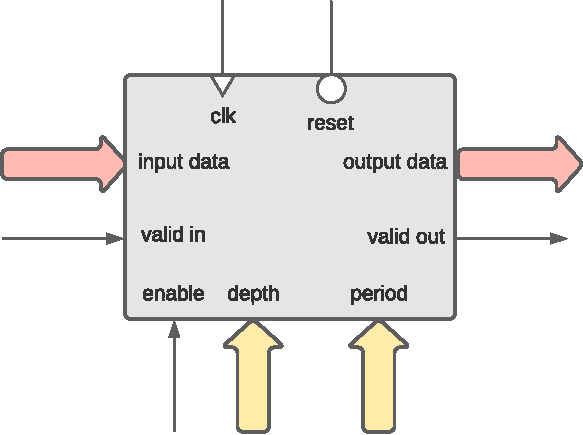
\includegraphics[scale=0.75]{img/diagrams/tremolo.pdf}
    \captionsetup{format=plain,justification=centering}
    \caption{Struktura wyprowadzeń bloku tremolo}
    \label{tremolo-structure}
\end{figure}
\vspace{0.5cm}

Implementacja generatora fali trójkątnej była dużo prostsza i~sprowadzała się do realizacji dwukierunkowego licznika. Gdy oba generatory zostały wdrożone\footnote{...oraz przetestowane z~wykorzystaniem dedykowanyc symulacjii}, realizacja efektu stała się formalnością. Jego architektura podzielona została na dwa procesy. Pierwszy z~nich odpowiada za generowanie fali modulującej. W~każdym takcie zegara wartość wewnętrznego licznika porównywana jest z~wartością na wejściu \verb|period|. Jeżeli są one równe, generowana jest następna próbka. W~przeciwnym wypadku licznik jest inkementowany. Drugi z~procesów monitoruje wejście \verb|valid in|. Gdy jego stan zostanie ustawiony na wysoki, próbka wejściowa oraz parametr \textit{depth} zostają przepisane do wewnętrznych buforów. Obliczenie wartości próbki wynikowej zgodnie z~ww. wzorem zachodzi asynchronicznie. Jako że iloczyn $d \times m[t]$ nie zawiera się w~przedziale $[0,1]$ koniecznym staje się przesunięcie wyniku tej operacji w~prawo o~liczbę bitów będącą sumą szerokości próbki generatora i~szerokości wejścia \verb|depth|. W~następnym takcie po zapisaniu buforów przetworzona próbka zostaje wystawiona na wyjście układu. Zastosowany rozdział obsługi LFO oraz przetwarzania sygnału wyjściowego pozwolił uniezależnić czas przetwarzania próbki wejściowej od czasu generowania próbek LFO. W~ten sposób udało się uzyskać opóźnienie na poziomie \textbf{1~cyklu}.

Wycinek symulacji przeprowadzonych dla efektu tremolo został przedstawiony na Rys. \ref{sim-tremolo}. Sygnał wejściowy to ponownie fala sinus o~częstotliwości $440$Hz. Wartość współczynnika \verb|period| dobrana została tak, aby uzyskać częstotliwość modulacji na poziomie $70$Hz. Współczynnik głębokości ustawiono na najwyższą wartość. Zastosowano modulację z~wykorzystaniem 8-bitowej fali trójkątnej. Analogiczne symulacje przeprowadzone zostały również dla drugiego typu modulacji. W~obu przypadkach układ wydaje się działać prawidłowo. 

\vspace{0.5cm}
\begin{figure}[ht]
    \centering
    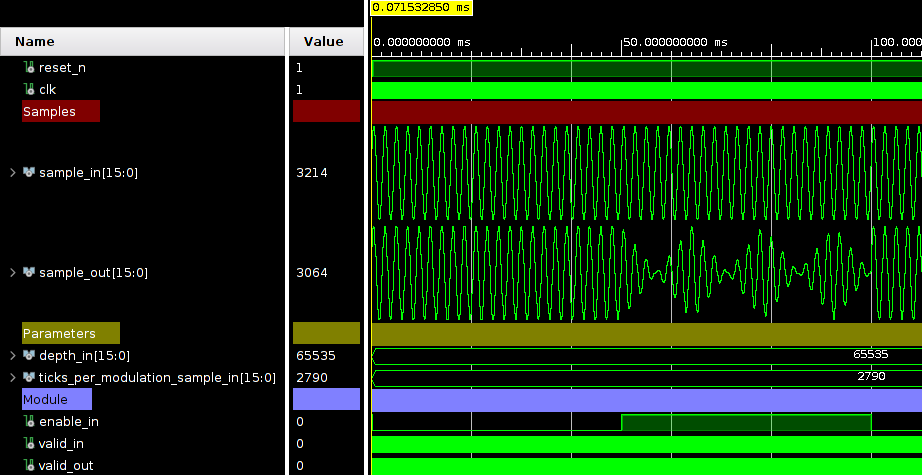
\includegraphics[width=\textwidth]{img/sim/tremolo_sim.png}
    \captionsetup{format=plain,justification=centering}
    \caption{Fragment symulacji działania efektu tremolo}
    \label{sim-tremolo}
\end{figure}
\vspace{0.5cm}